\subsection{Verification of Contact Models \label{Chapter 2: ABAQUS Applied to Contact Models} }

Applying ABAQUS to assessing simple contact models of indentation provides a robust validation of the FEM approach. Three types of indenters were used for the simulations: conical, spherical, and spherically-capped conical. The behaviour of each indenter was characterized and compared with the theoretical indentation models: Hertz\cite{kontomaris2018hertz} and Dimitriadis\cite{DIMITRIADIS20022798} for spherical indenters, and Sneddon\cite{han2021modified} for conical indenters (Details of the models are shown in the Appendix \ref{Appendix: Models of Indentation in Atomic Force Microscopy}). The simulations focused on the elastic indentation of both elastic half-spaces/planes of varying depths and elastic spheres of varying radii. For computational efficiency, asymmetric models centered around the indentation axis (y-axis) were used, as shown in Figure \ref{fig: ABAQUS-Model-Setup}. Indenters were modelled as rigid (incompressible) parts restricted to the y-direction. The elastic half-spaces were fixed at the base, while the elastic spheres had a fixed, rigid base beneath them. The model surfaces were simulated as homogeneous, isotropic elastic materials with Young's modulus and Poisson ratio of $1000 KPa$ and 0.3, respectively. These values were chosen as they are typical biomolecule values, and as such, dimensions were given in nm and pN (although somewhat arbitrary as analysis is dimensionless).

\begin{figure}[H]
\centering

    \begin{subfigure}{0.3\textwidth}
        \centering
        \caption{\label{fig: Cone-Sphere-ABAQUS-setup}}
        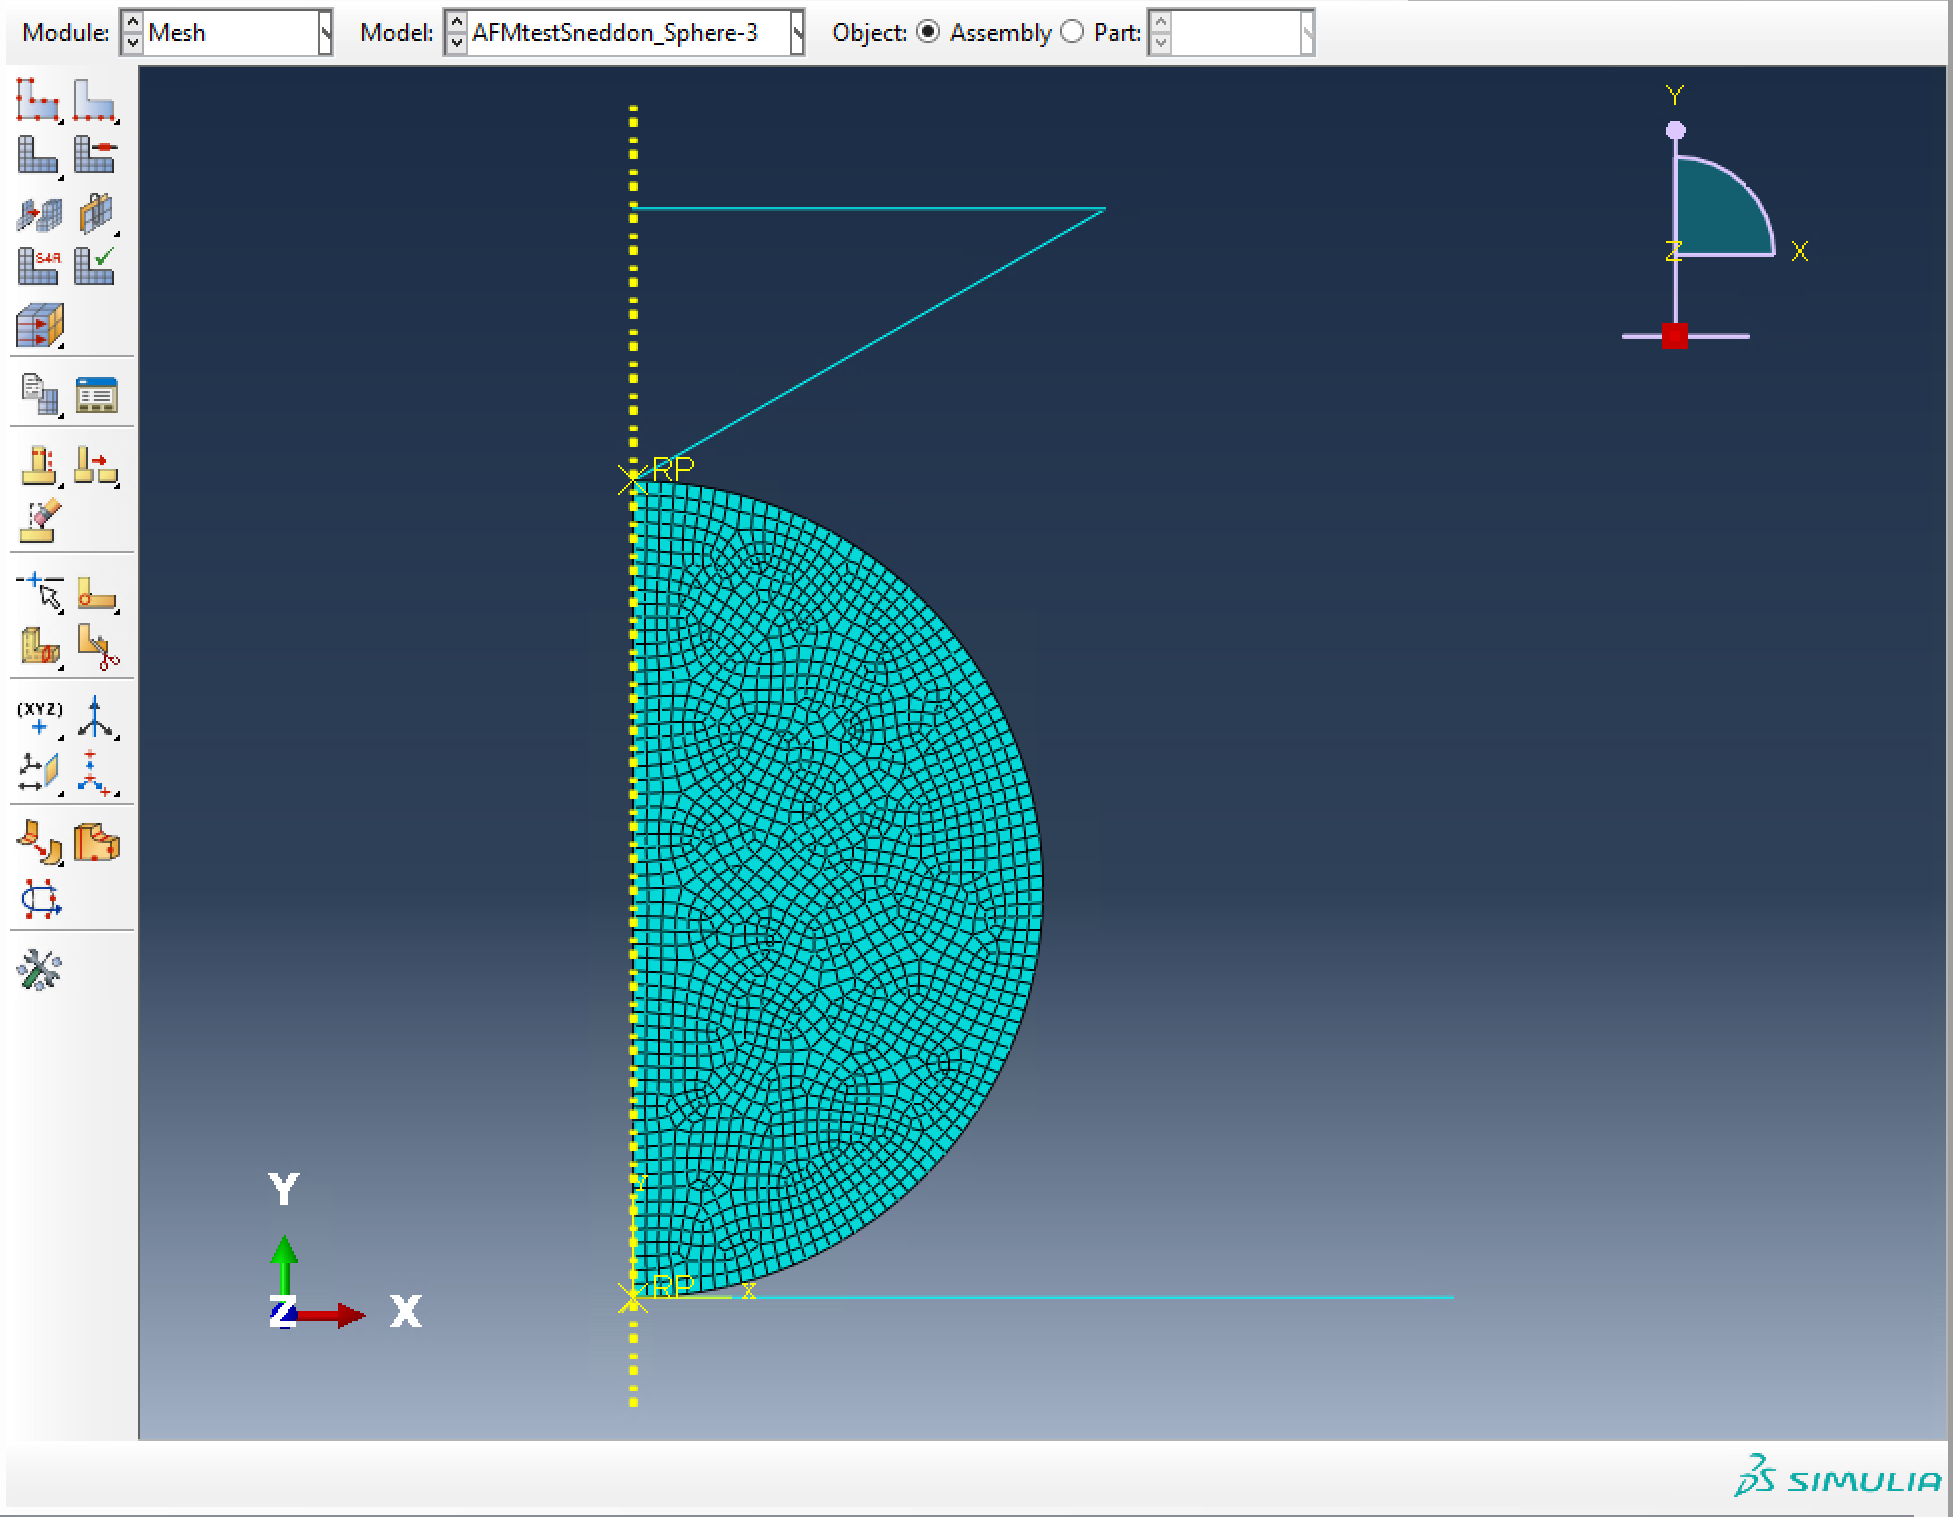
\includegraphics[width=1\linewidth]{Figures/Cone-Sphere-ABAQUS-setup.png}
    \end{subfigure}
    \hfill     
    \begin{subfigure}{0.3\textwidth}
        \centering
        \caption{\label{fig: Sphere-Sphere-ABAQUS-setup}}
        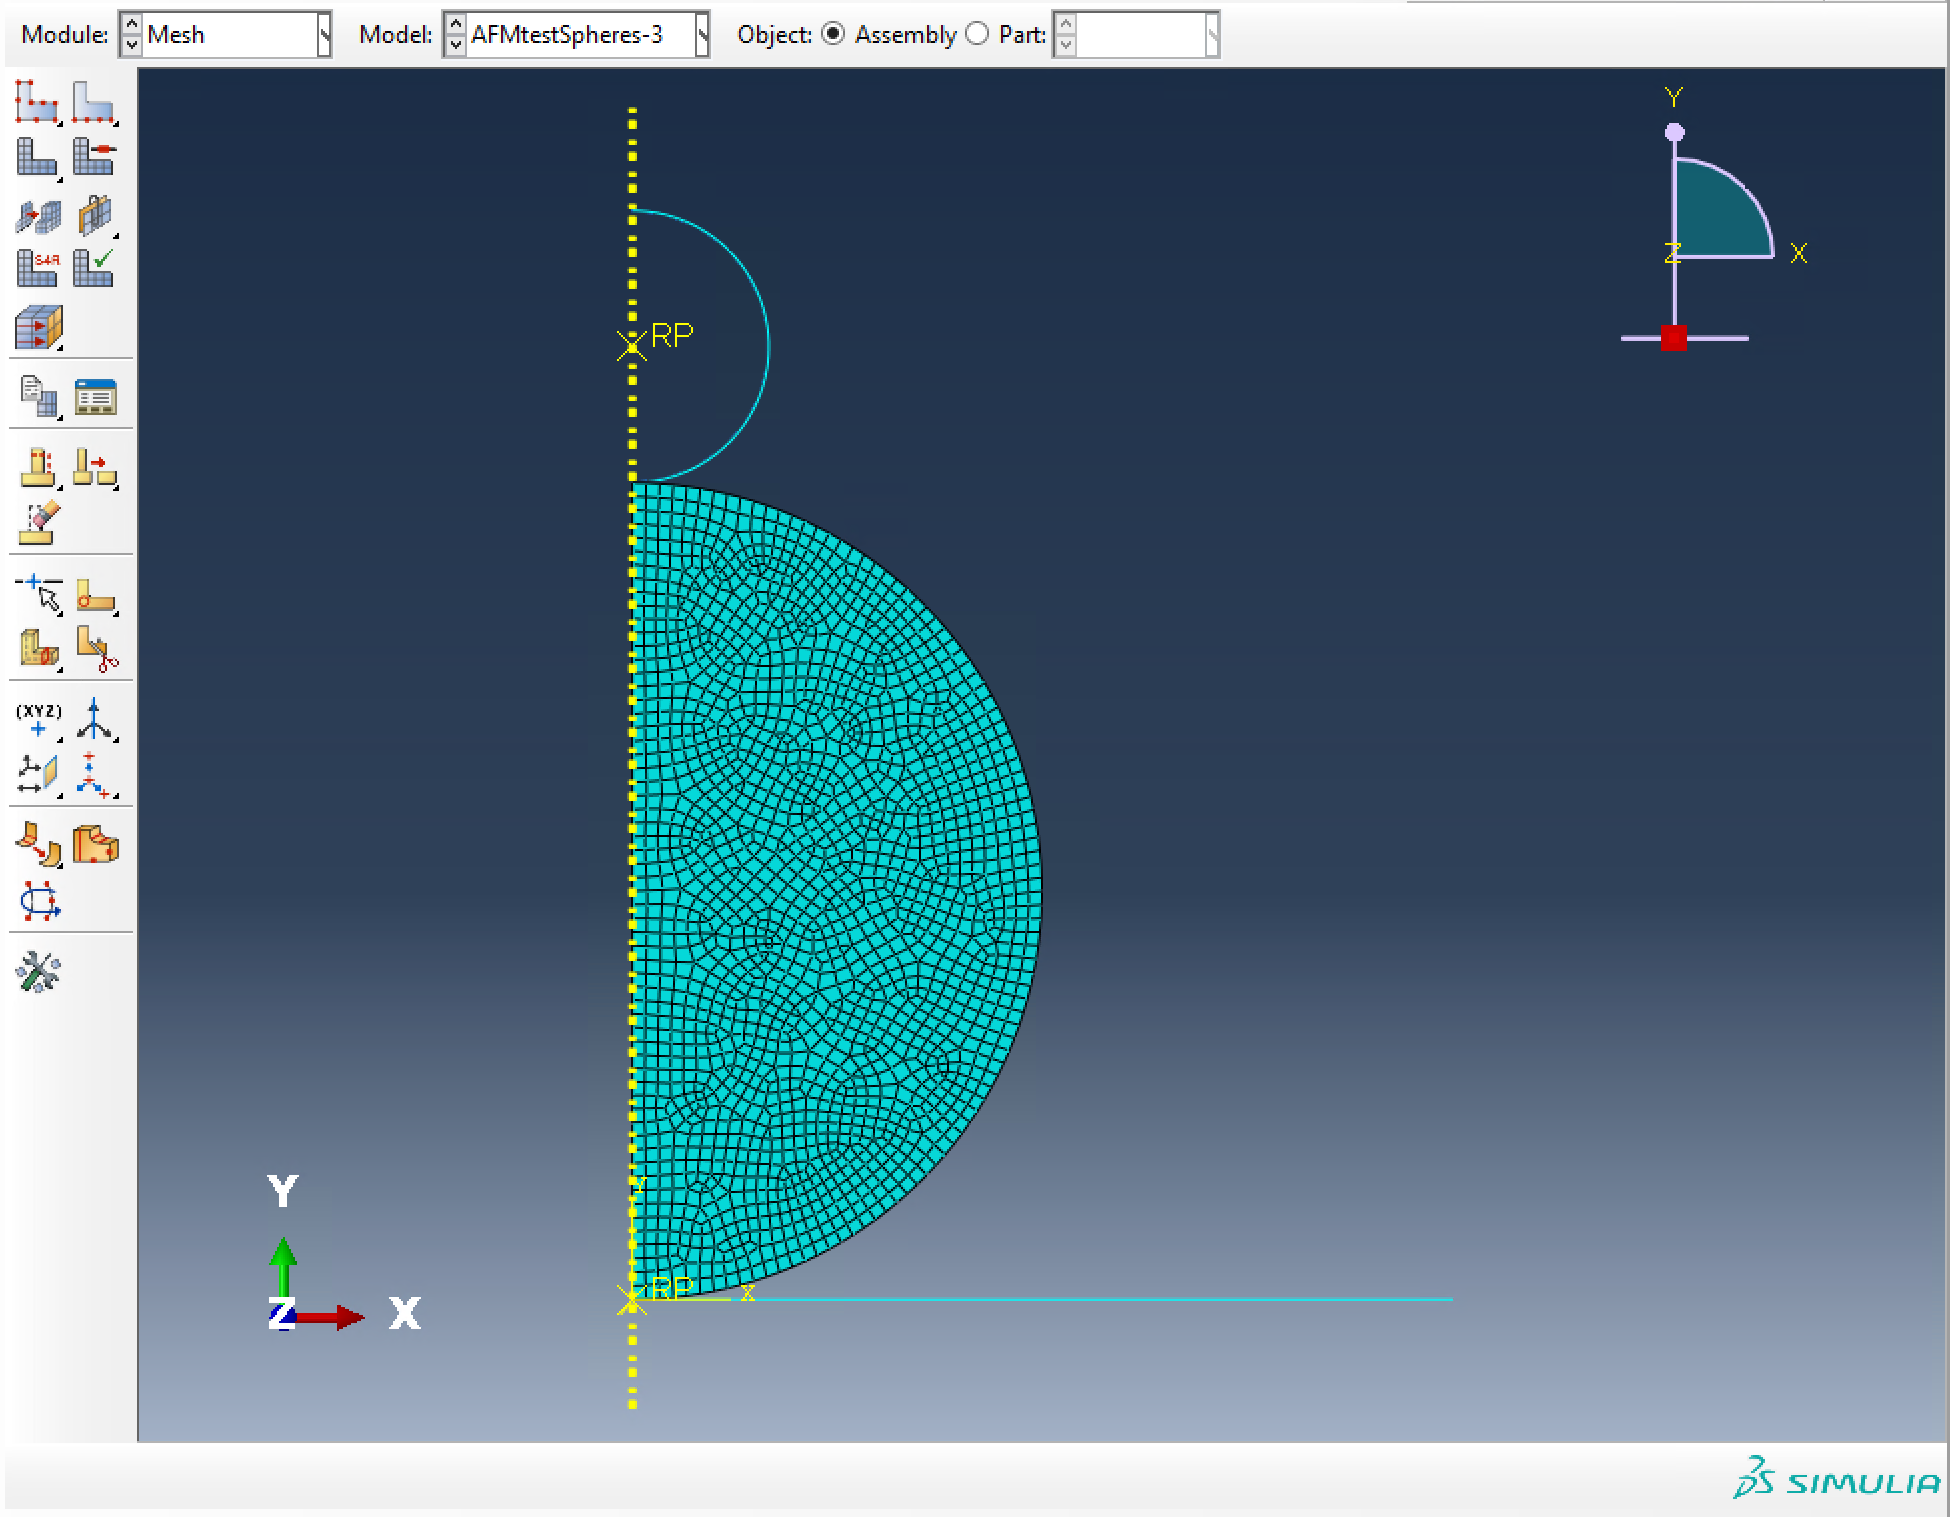
\includegraphics[width=1\linewidth]{Figures/Sphere-Sphere-ABAQUS-setup.png}
    \end{subfigure}
    \hfill
    \begin{subfigure}{0.3\textwidth}
        \centering
        \caption{\label{fig: Capped-Sphere-ABAQUS-setup}}
        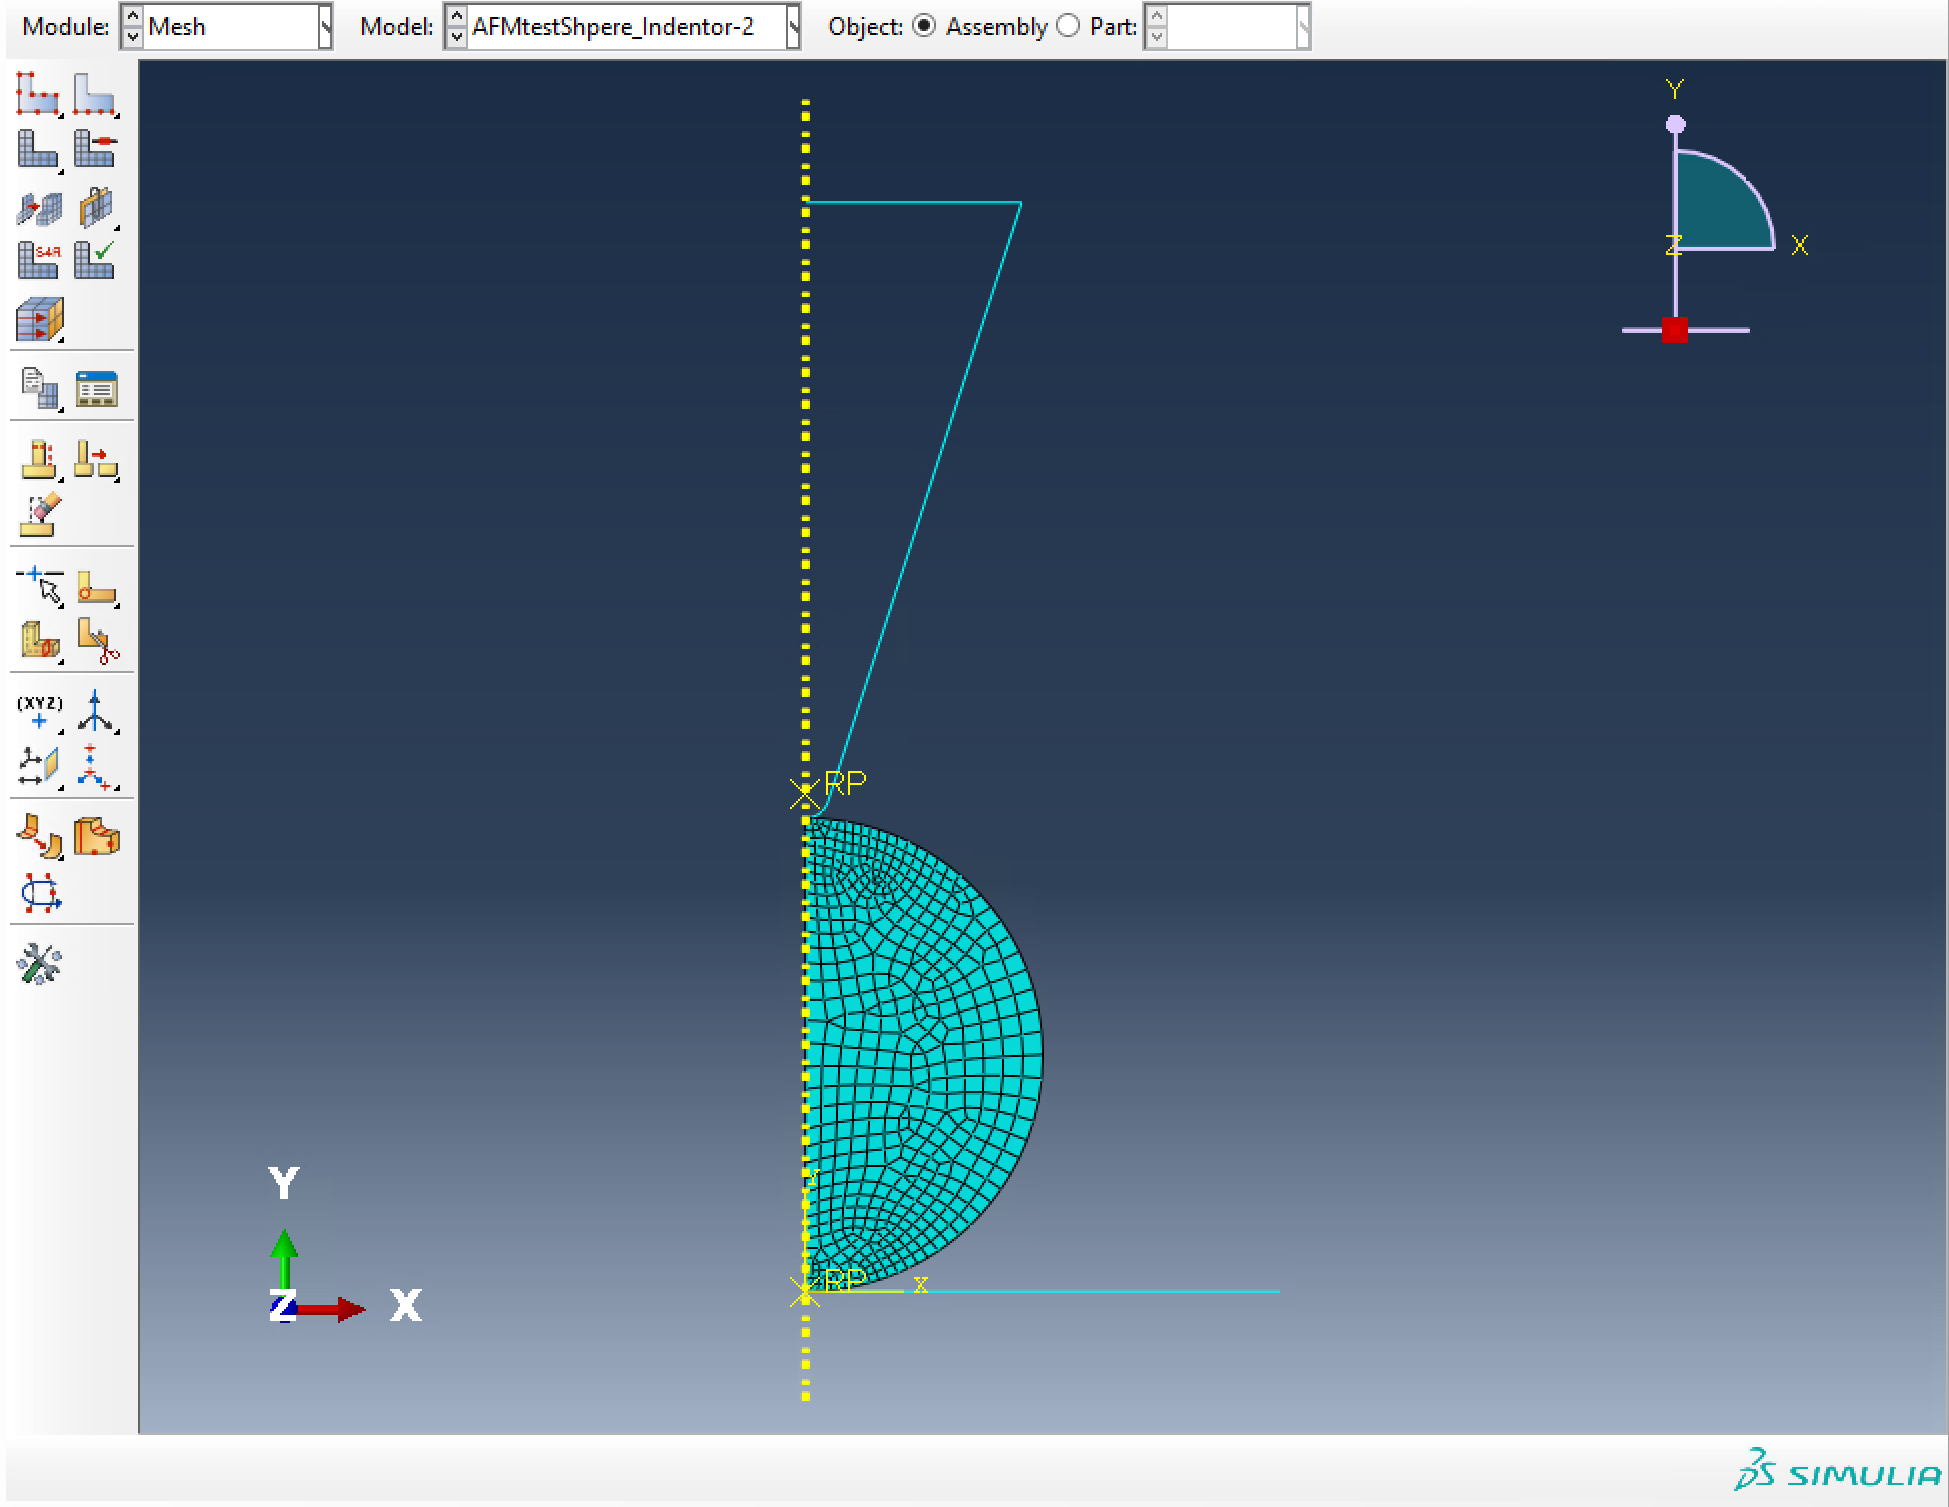
\includegraphics[width=1\linewidth]{Figures/Capped-Sphere-ABAQUS-setup.png}
    \end{subfigure}   
    
    \hfill
    
    \begin{subfigure}{0.3\textwidth}
        \centering
        \caption{\label{fig: Cone-Plane-ABAQUS-setup}}
        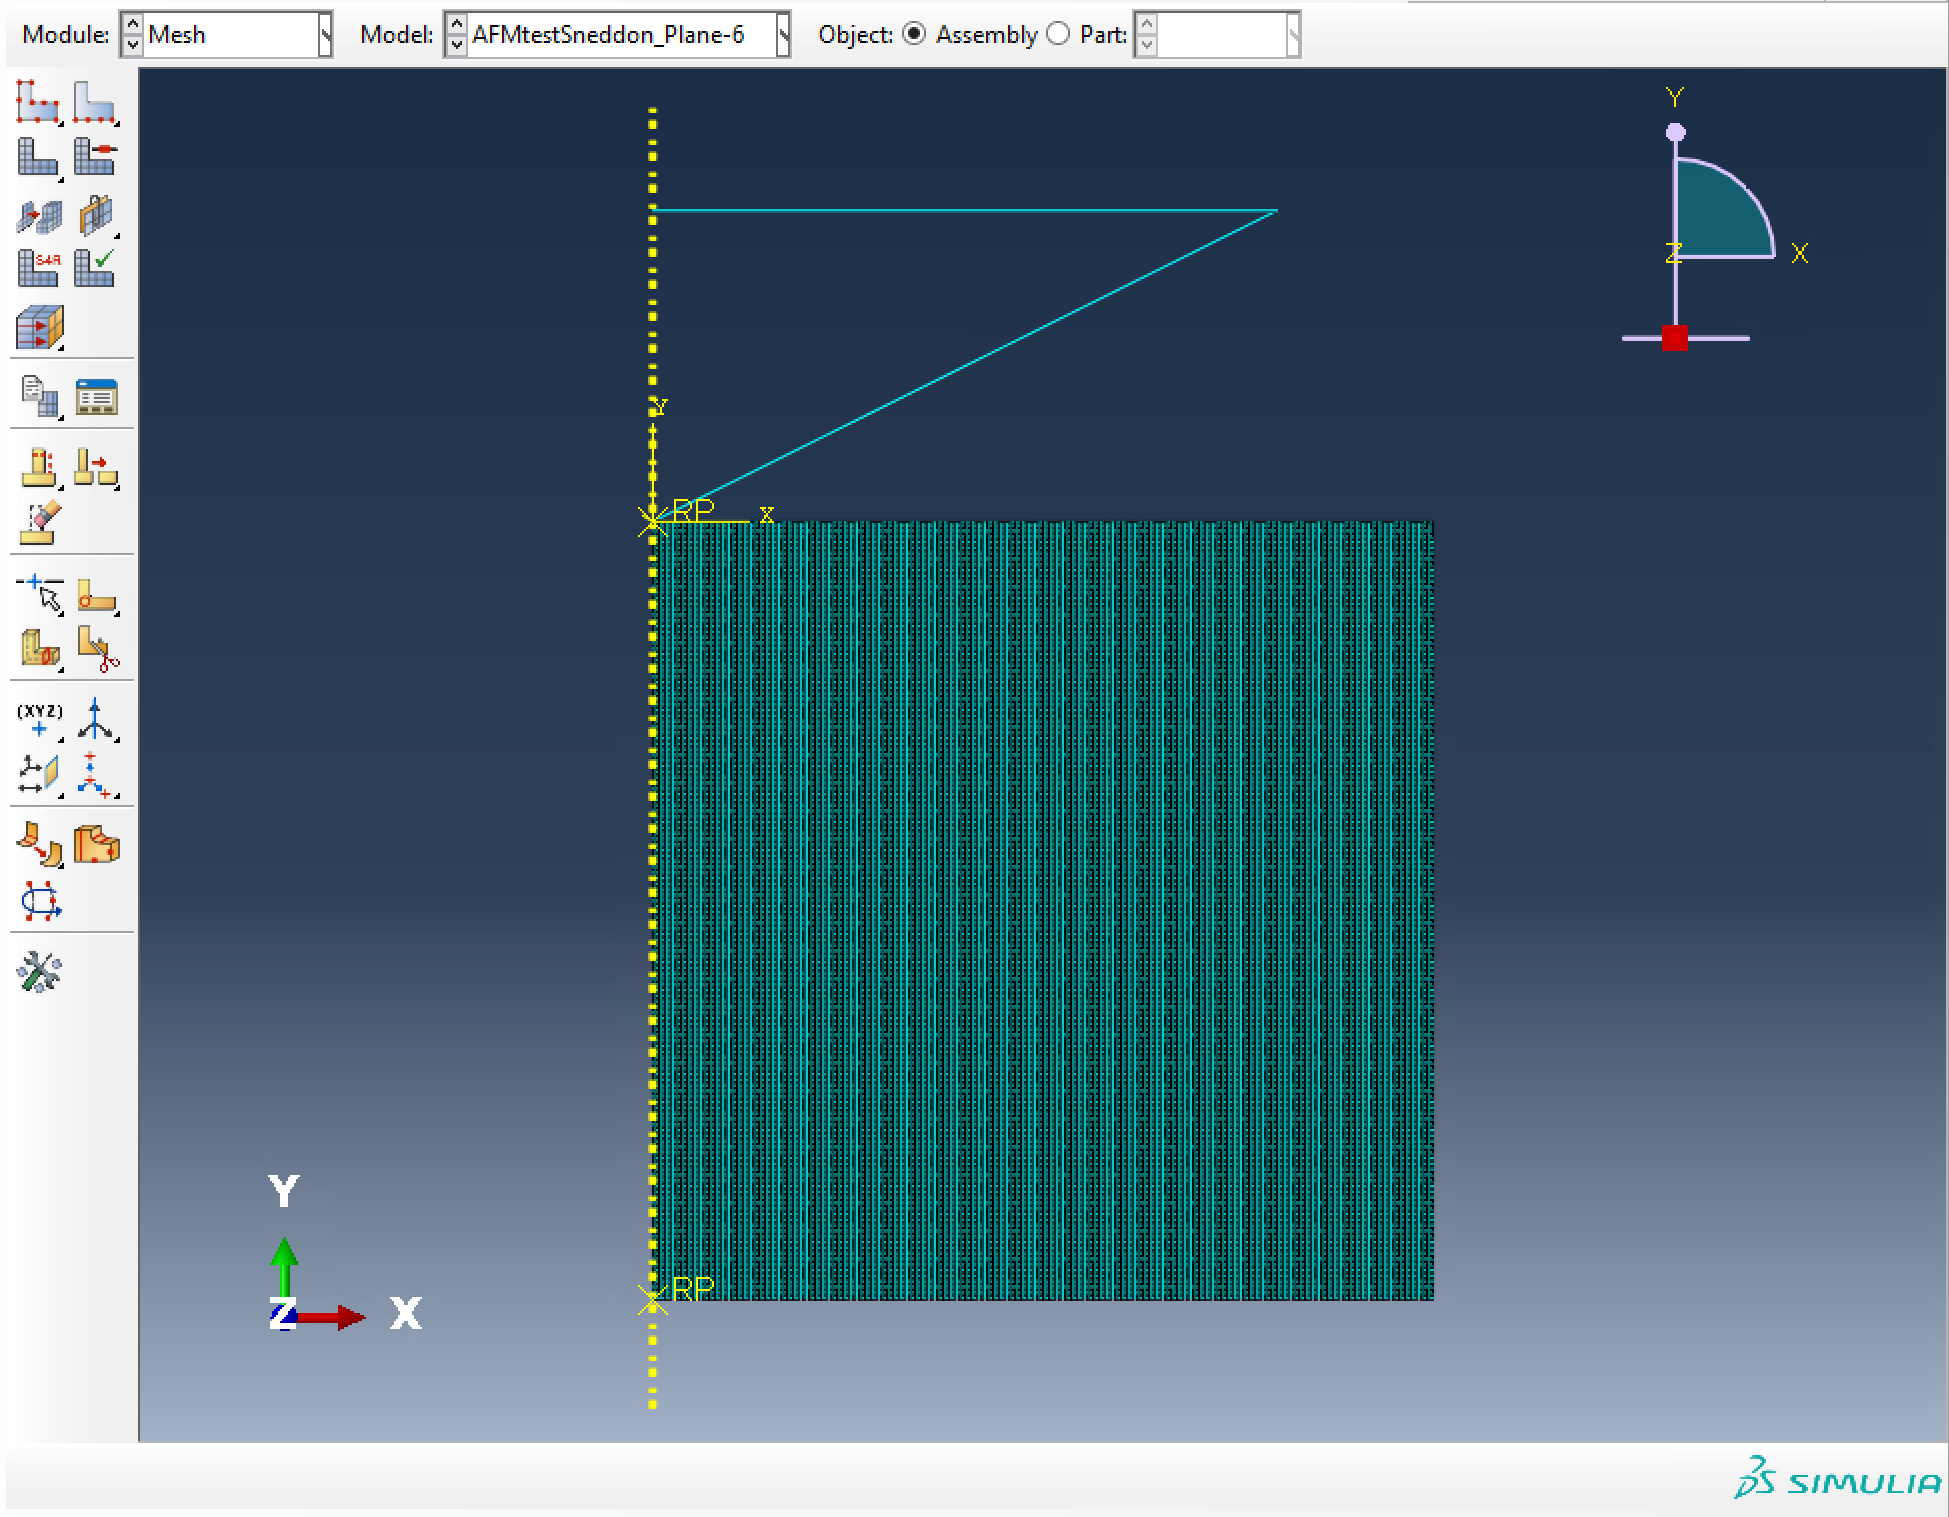
\includegraphics[width=1\linewidth]{Figures/Cone-Plane-ABAQUS-setup.png}
    \end{subfigure}  
    \hfill  
    \begin{subfigure}{0.3\textwidth}
        \centering
        \caption{\label{fig: Sphere-Plane-ABAQUS-setup}}
        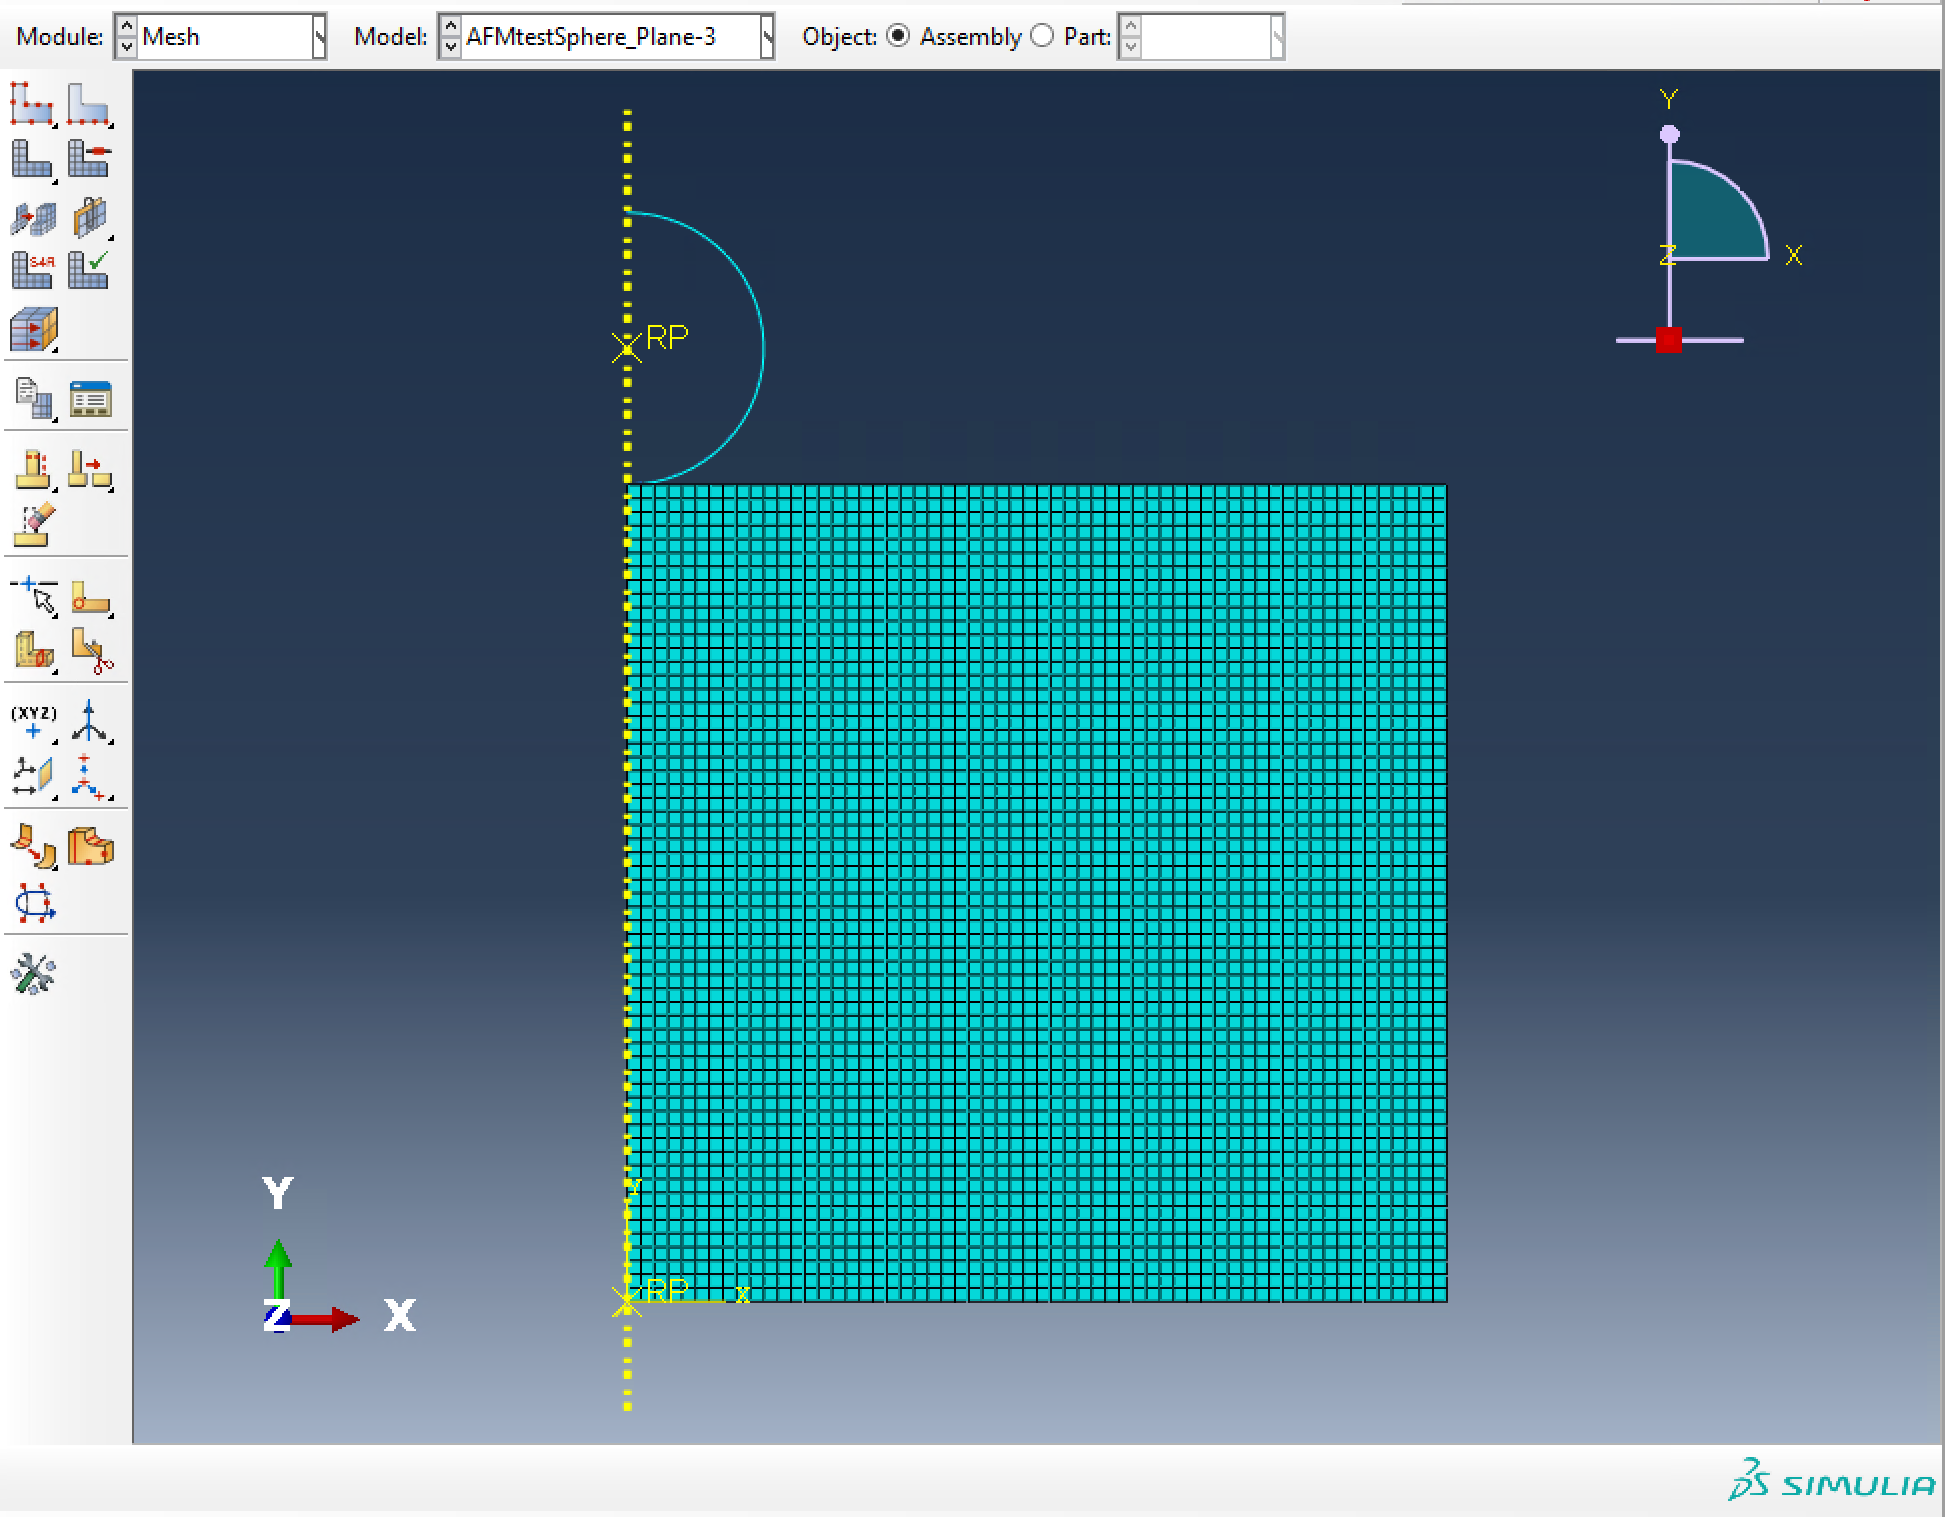
\includegraphics[width=1\linewidth]{Figures/Sphere-Plane-ABAQUS-setup.png}
    \end{subfigure}  
    \hfill
    \begin{subfigure}{0.3\textwidth}
        \centering
        \caption{\label{fig: Capped-Plane-ABAQUS-setup}}
        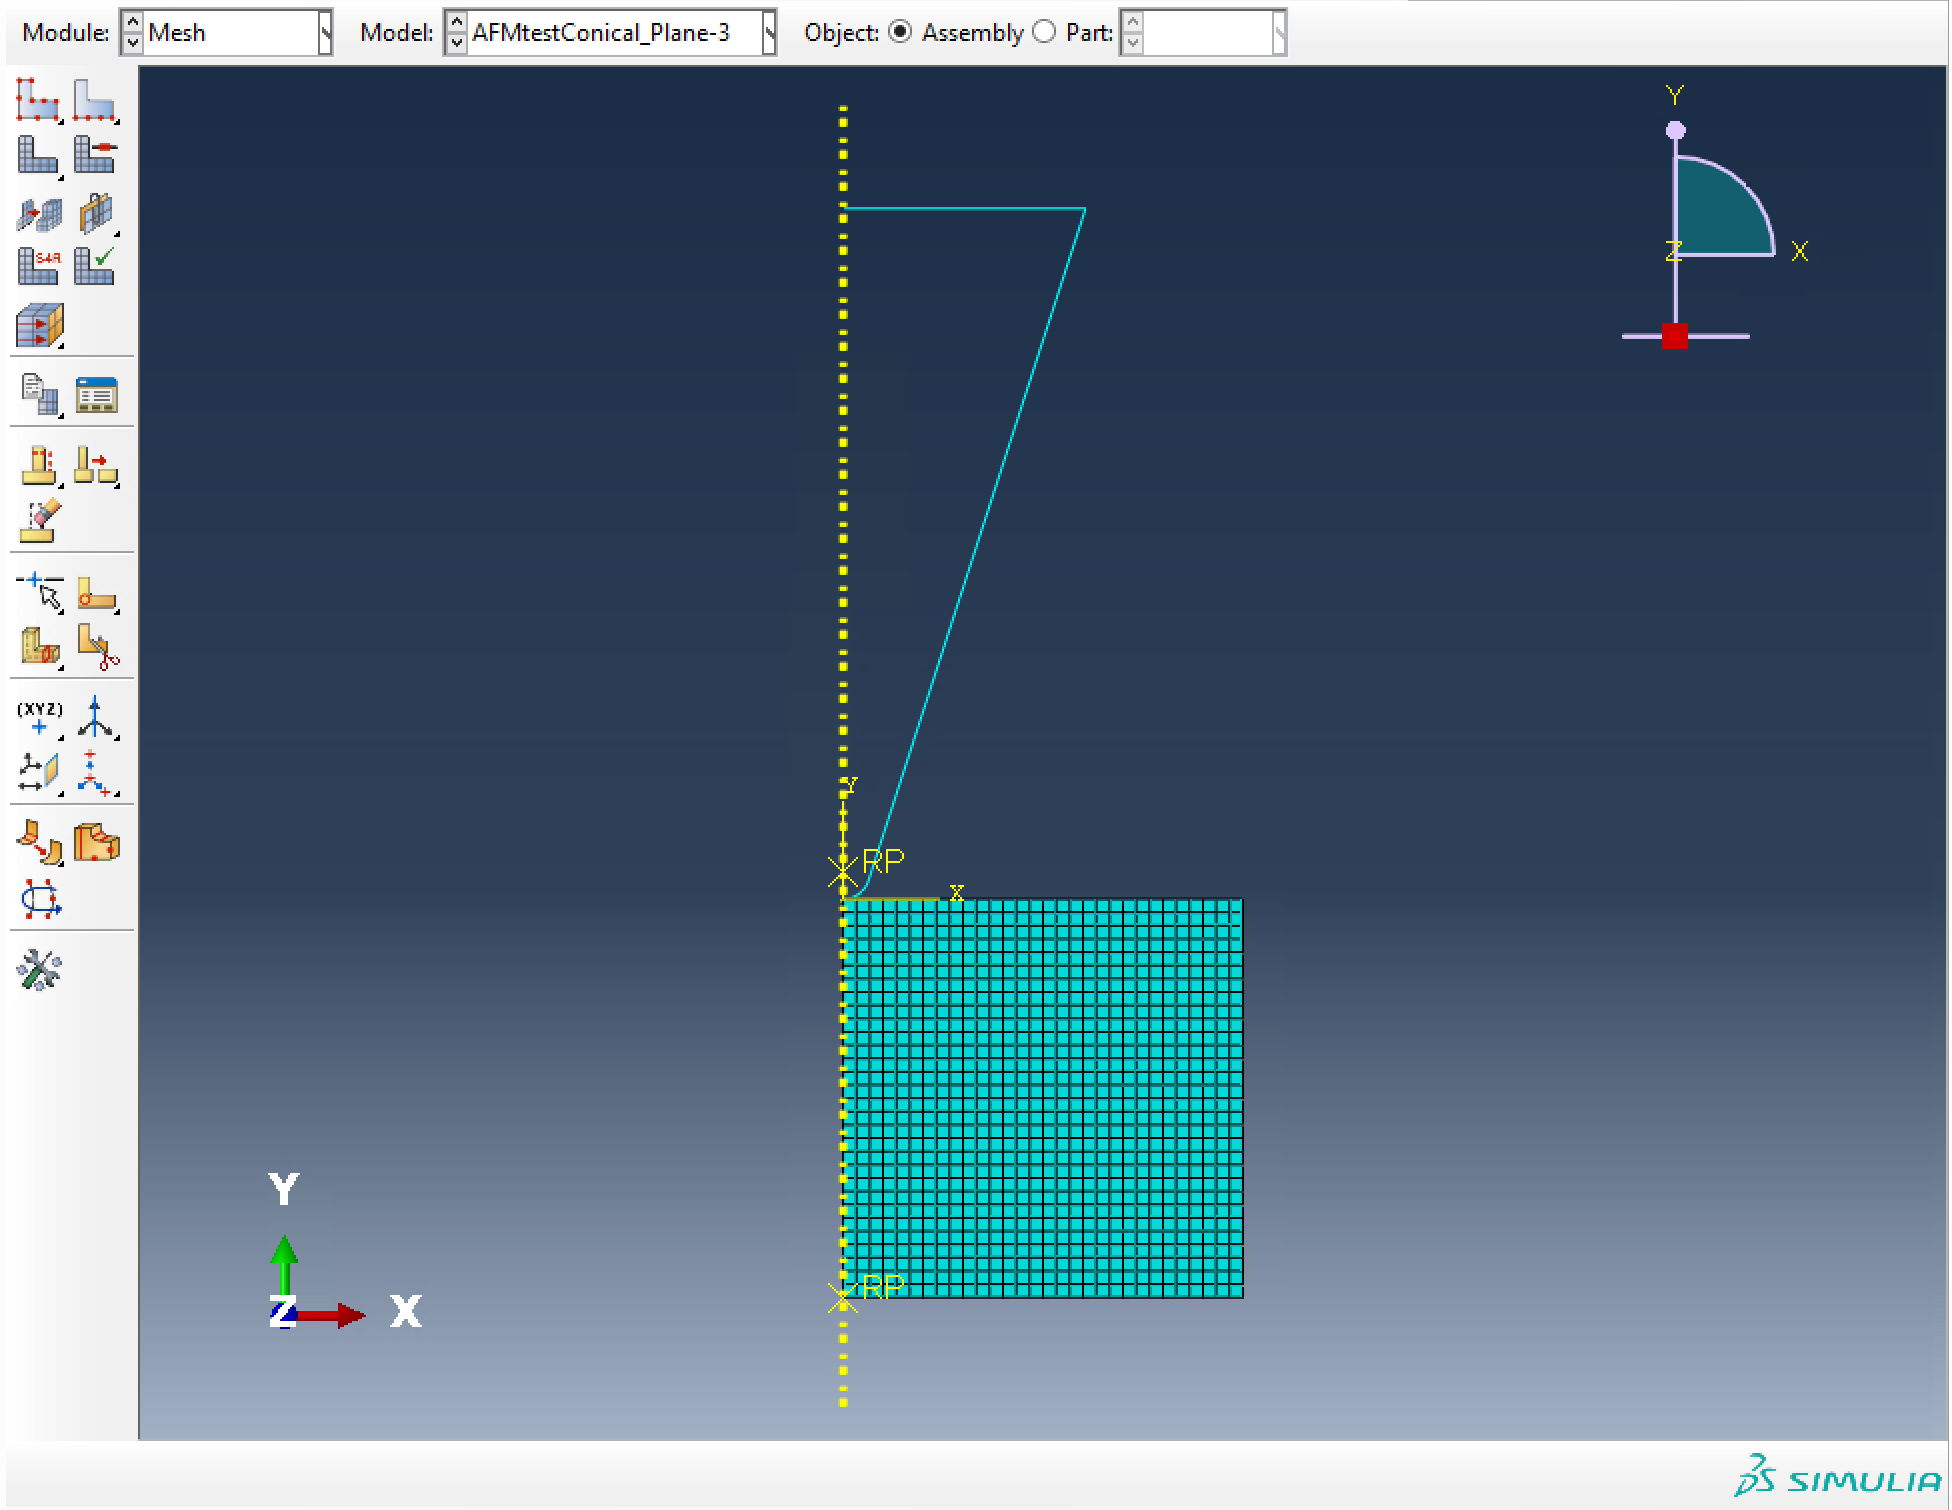
\includegraphics[width=1\linewidth]{Figures/Capped-Plane-ABAQUS-setup.png}
    \end{subfigure}

    
    \caption{\label{fig: ABAQUS-Model-Setup}ABAQUS model assembly from elastic indentation tests. Elastic half-spaces were modelled asymmetrically using rectangles. Elastic spheres were modelled using semi-circles with a rigid base beneath. Models include (A) Conical indentation of an elastic sphere. (B) Spherical indentation of an elastic sphere. (C) Spherically-capped conical indentation of an elastic sphere. (D) Conical indentation of an elastic half-space. (E) Spherical indentation of elastic half-space. (F) Spherically-capped conical indentation of an elastic half-space.}
\end{figure}

The contact was modelled as a "surface-to-surface" type with "hard" (nonadhesive) properties in the normal direction and "rough" (non-slip) Coulomb friction in the tangential direction. Vertical force and indentation data was sampled via reference points at the centre of the indenter. As it is a rigid part, ABAQUS maps the forces and displacement of the surface of the part to the reference point. For elastic spheres, Double Contact Models\cite{dokukin2013quantitative,glaubitz2014novel} were required to account for more complex dynamics discussed in the results. Simulations were quasi-static computations using an implicit algorithm and approximately 30000 tetrahedral (R3D10) elements. The simulation data was exported to Python and scipy.curve\_fit module was used to fit the desired contact model. Example scripts in Appendix \ref{Appendix: ABAQUS Script}.
